\documentclass[a4paper,titlepage]{article}
\usepackage[utf8]{inputenc}
\usepackage{fullpage}
\usepackage{indentfirst}
\usepackage[per-mode=symbol]{siunitx}
\usepackage{listings}
\usepackage{graphicx}
\usepackage{color}
\usepackage{amsmath}
\usepackage{array}
\usepackage[hidelinks]{hyperref}
\usepackage[format=plain,font=it]{caption}
\usepackage{subcaption}
\usepackage{standalone}
\usepackage[nottoc]{tocbibind}
\usepackage[noabbrev,capitalize,nameinlink]{cleveref}
\usepackage{listings}
\usepackage{xspace}
\usepackage{tikz}
\usepackage{circuitikz}
\usepackage{titlesec}
\usepackage[cache=false]{minted}
\usepackage{booktabs}
\usepackage{csvsimple}
\newcommand{\MATLAB}{\textsc{Matlab}\xspace}
\usepackage{siunitx}
\usepackage[super]{nth}
\usepackage[titletoc]{appendix}

% Custom commands
\newcommand\numberthis{\addtocounter{equation}{1}\tag{\theequation}}
\newcommand{\code}[1]{\texttt{#1}}
\newcolumntype{P}[1]{>{\centering\arraybackslash}p{#1}}

\setminted{linenos,breaklines,fontsize=auto}

%\titleformat*{\section}{\normalsize\bfseries}
%\titleformat*{\subsection}{\small\bfseries}
\renewcommand{\thesubsection}{\thesection.\alph{subsection}}
\providecommand*{\listingautorefname}{Listing}
\newcommand*{\Appendixautorefname}{Appendix}

%opening
\title{\textbf{ECSE 543: Numerical Methods} \\ Assignment 1}
\author{Wenjie Wei \\ 260685967}
\date{\today}

\begin{document}
	\sloppy
	
	\maketitle
	
	\tableofcontents
	
	
	\twocolumn
	
	\section{Introduction}
	
	All programs in this assignment are written and compiled with Python 3.6. This report is structured so that the individual problems are answered in respective sections. The python codes used to solve the assignment problems are attached in the appendices, with the file names labeled at the top of the code segments.
	
	\section{Choleski Decomposition}
		\subsection{Choleski Implementation}
			The implementation of Choleski decomposition is shown in Listing \ref{lst:choleski}. There are two methods defined in \mintinline{python}{choleski.py}: \mintinline{python}{check_choleski(A, b, x)} and \mintinline{python}{choleski_decomposition(A, b)}. The latter method takes two matrices \mintinline{python}{A} and \mintinline{python}{b} as arguments, and returns \mintinline{python}{x} as the computational result of the decomposition. The first method takes these three matrices as arguments, and performs matrix production to check the result of
			$$
				Ax = b
			$$ 
			The precision of the equality is set to 0.001, as the program may end up with results with uncertainties with a quantity level of $10^{-8}$.
			
		\subsection{Simple Tester Matrices}
			To test the functionality of the program, we construct tester matrices with size varying from 2 to 10. The matrices are constructed to be symmetric, positive definite. 
			
			To construct the testing matrices, start from the fact that $A$ must be symmetric, positive definite if cholesky decomposition succeeds. Thus, we do the reverse process by constructing a lower-triangular matrix $L$, and thus obtain $A$ by $A = LL^T$. Below are several test matrices, and the results of the running are shown in Figures \ref{chol_1_result} and \ref{chol_2_result}.
			
			Testing matrices 1:
			$$
				\begin{bmatrix}
				15 & -5 & 0 & -5 \\
				-5 & 12 & -2 & 0 \\
				0 & -2 & 6 & -2 \\
				-5 & 0 & -2 & 9
				\end{bmatrix} x =
				\begin{bmatrix}
				115\\
				22\\
				-51\\
				13
				\end{bmatrix}
			$$
			Output results:
			\begin{figure}[!h]
				\centering
				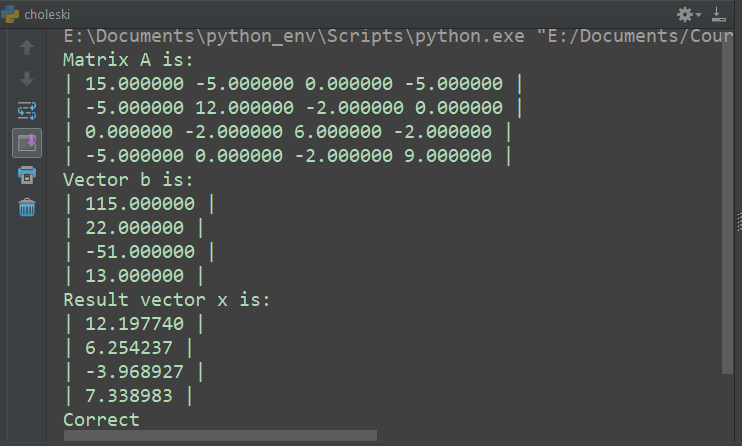
\includegraphics[width=\linewidth]{chol_1_result}
				\caption{Result of the First Choleski Decomposition Test}
				\label{chol_1_result}
			\end{figure}
		
			Testing matrix 2:
			$$
				\begin{bmatrix}
				38 & 23& 31& 22& 29& 25& 31\\
				23& 44& 36& 27& 35& 24& 33\\
				31& 36& 65& 36& 45& 34& 45\\
				22& 27& 36& 46& 29& 15& 27\\
				29& 35& 45& 29& 52& 32& 39\\
				25& 24& 34& 15& 32& 37& 36\\
				31& 33& 45& 27& 39& 36& 65
				\end{bmatrix}x = \begin{bmatrix}
				13\\4\\7\\23\\17\\5.8\\10
				\end{bmatrix}
			$$
			Output results:
			\begin{figure}[!h]
				\centering
				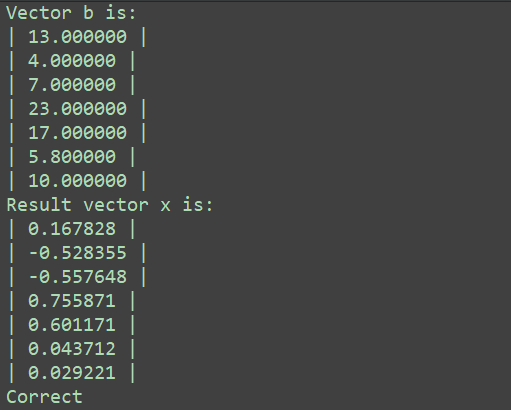
\includegraphics[width=\linewidth]{chol_2_result}
				\caption{Result of the Second Choleski Decompostion Test}
				\label{chol_2_result}
			\end{figure}
		\subsection{Testing of $Ax = b$}
			The outputs of two testing cases are shown in Figures \ref{chol_1_result} and \ref{chol_2_result} in the previous section. In the program implemented, there is a simple checking method which does a dot product of $A$ and $x$ and check if the results match the entries entered for $b$. Note that because of the reason of the Python interpreter, there is a tiny error with a quantity of $10^{-10}$, therefore the precision is set to $10^{-5}$ to check the validity of the computation.
		\subsection{Linear Resistive Networks}
			Linear resistive networks are now able to be solved by the Choleski decomposition implemented in the previous parts. Listing \ref{lst:linear_networks} shows the implementation of reading a circuit file with data organized in a .csv file.
			
			\begin{figure}[!h]
				\centering
				\begin{circuitikz}[american voltages]
					\draw
					(0, 0) to [V, *-*] (0, 4)
					(0, 4) to [R, l=$20\Omega$, *-*] (3, 4) node[label={[font=\footnotesize]above:$V_1$}]{}
					to [R, l=$10\Omega$, *-*] (3, 2)node[label={[font=\footnotesize]left:$V_2$}]{}
					to [R, l=$30\Omega$, *-*] (6, 2)
					to [R, l=$30\Omega$, *-*] (6, 0)
					(3, 4) to [short, *-*] (6, 4)
					to [R, l=$10\Omega$, *-*] (6, 2)node[label={[font=\footnotesize]right:$V_3$}]{}
					(3, 2) to [R, l=$30\Omega$, *-*] (3, 0)
					to [short, *-*] (6, 0)
					to [short, *-*] (0, 0)
					(3, 0) node[ground]{}
					;
				\end{circuitikz}
				\caption{Test Circuit 5}
				\label{tc5}
			\end{figure}
			
			\begin{figure}[!h]
				\centering
				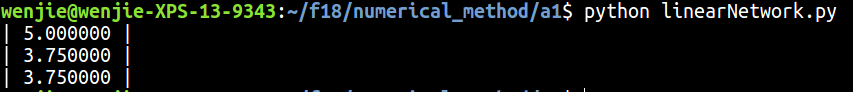
\includegraphics[width=\linewidth]{tc5_result}
				\caption{Result of the Testing Circuit 5}
				\label{tc5_result}
			\end{figure}
			
			Take the 5th circuit provided by the TA for example, the circuit is shown in Figure \ref{tc5}, and the result of the running of the program on this circuit is shown in Figure \ref{tc5_result}.
						
			The data of the circuit are organized in the way shown in Figure \ref{lin_network_org}.
			\begin{figure}[!h]
				\centering
				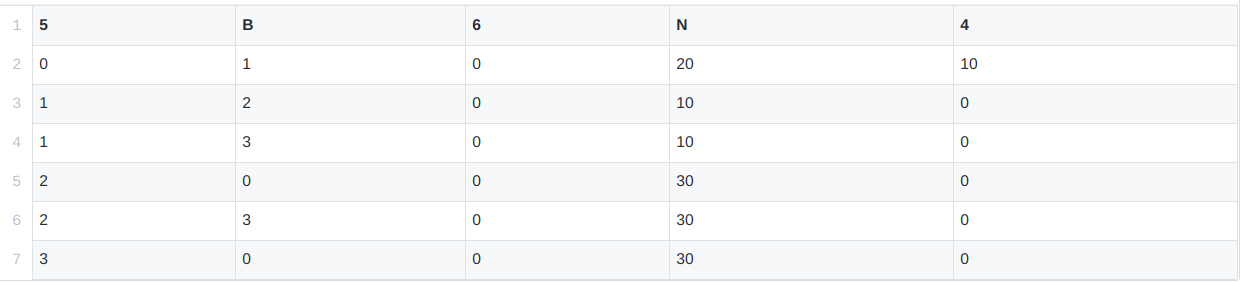
\includegraphics[width=\linewidth]{lin_network_org}
				\caption{Circuit File Organizations}
				\label{lin_network_org}
			\end{figure}
			The first line shows the general information about the circuit, such as the circuit ID (the example shown in the figure is the 5th test circuit), number of branches, and number of nodes. The lines followed are the data of the branches, which contains the following data: the starting node, the end node, the current source $J$, the resistance $R$, and the voltage source $E$.
			
			The convention of the input files should be well defined. In the program used for this test circuit, define the positive current direction is flowing from the start node to the end node. Current source must deliver positive current to the start node and the voltage source should deliver positive current to the end node. Following the conventions listed above, the program should be able to output desired node voltages in matrix form. 
			
			To verify the reliability of the program, four more simple test circuits are constructed. The input file as well as the result of the calculations are attached immediately after the circuit diagrams. The test runs below are proving that the program runs correctly as long as appropriate input files are passed into.
			\subsubsection{Testing Circuit 1}
				Figures \ref{tc1} and \ref{tc1_result} show the first test circuit. The desired output at node 1 can be calculated as $V_1 = 5V$, and the program is outputting the correct result.
				\begin{figure}[!h]
					\centering
					\begin{circuitikz}[american voltages]
						\draw
						(0, 0) to [V, l=$10V$, *-*] (0, 2)
						to [R, l=$10\Omega$, *-*] (2, 2) node[label={[font=\footnotesize]above:$V_1$}]{}
						to [R, l=$10\Omega$, *-*] (2, 0) node[ground]{}
						to [short, *-*] (0, 0)
						;
					\end{circuitikz}
					\caption{Test Circuit 1}
					\label{tc1}
				\end{figure}
				\begin{figure}[!h]
					\centering
					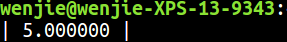
\includegraphics[width=\linewidth]{tc1_result}
					\caption{Output Result of the Testing Circuit 1}
					\label{tc1_result}
				\end{figure}
			\subsubsection{Testing Circuit 2}
				Figures \ref{tc2} and \ref{tc2_result} below show the testing circuit 2 and its result. The expected result is $V_1 = 50V$.
				\begin{figure}[!h]
					\centering
					\begin{circuitikz}[american voltages, american currents]
						\draw
						(0, 0) to [V, l=$10V$, *-*] (0, 2)
						to [short, *-*] (2, 2) node[label={[font=\footnotesize]above:$V_1$}]{}
						to [R, l=$10\Omega$, *-*] (2, 0) node[ground]{}
						to [short, *-*] (0, 0)
						(2, 0) to [short, *-*] (4, 0)
						to [I, i_>=$10A$, *-*] (4, 2)
						to [short, *-*] (2, 2)
						;
					\end{circuitikz}
					\caption{Test Circuit 2}
					\label{tc2}
				\end{figure}
				\begin{figure}[!h]
					\centering
					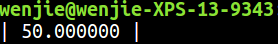
\includegraphics[width=\linewidth]{tc2_result}
					\caption{Output Result of the Testing Circuit 2}
					\label{tc2_result}
				\end{figure}
			\subsubsection{Testing Circuit 3}
				Figures \ref{tc3} and \ref{tc3_result} below show the results of the testing circuit 3. The expected result of the circuit is $V_1 = 55V$.
				\begin{figure}[!h]
					\centering
					\begin{circuitikz}[american voltages, american currents]
						\draw
						(0, 0) to [V, l=$10V$, *-*] (0, 2)
						to [R, l=$10\Omega$, *-*] (2, 2) node[label={[font = \footnotesize] above:$V_1$}]{}
						to [R, l=$10\Omega$, *-*] (2, 0) node[ground]{}
						to [short, *-*] (0, 0)
						(2, 0) to [short, *-*] (4, 0)
						to [I, i_>=$10A$, *-*] (4, 2)
						to [short, *-*] (2, 2)
						;
					\end{circuitikz}
					\caption{Test Circuit 3}
					\label{tc3}
				\end{figure}
				\begin{figure}[!h]
					\centering
					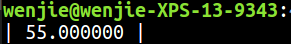
\includegraphics[width=\linewidth]{tc3_result}
					\caption{Output Result of the Testing Circuit 3}
					\label{tc3_result}
				\end{figure}
			\subsubsection{Testing Circuit 4}
				Figures \ref{tc4} and \ref{tc4_result} below show the results of the testing circuit 4. The expected results of the circuit is $V_1 = 20V$ and $V_2 = 35V$.
				\begin{figure}[!h]
					\centering
					\begin{circuitikz}[american voltages, american currents]
						\draw
						(0, 0) to [V, l=$10V$, *-*] (0, 2)
						to [R, l=$10\Omega$, *-*] (2, 2) node[label={[font = \footnotesize] above:$V_1$}]{}
						to [R, l=$5\Omega$, *-*] (4, 2) node[label={[font = \footnotesize] above:$V_2$}]{}
						(4, 0)node[ground]{} to [R, l=$5\Omega$, *-*] (4, 2)
						(4, 0) to [short, *-*] (2, 0)
						to [R, l=$10\Omega$, *-*] (2, 2)
						(2, 0) to [short, *-*] (0, 0)
						(4, 0) to [short, *-*] (5, 0)
						to [I, i_>=$10A$, *-*] (5, 2)
						to [short, *-*] (4, 2)
						;
					\end{circuitikz}
					\caption{Test Circuit 4}
					\label{tc4}
				\end{figure}
				\begin{figure}[!h]
					\centering
					
					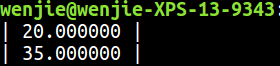
\includegraphics[width=\linewidth]{tc4_result}
					\caption{Output Result of the Testing Circuit 4}
					\label{tc4_result}
				\end{figure}
			
	\section{Resistor Mesh Network}
		\subsection{Implementation}
			The implementation of the program is shown in the appendix as Listing \ref{lst:linear_networks}. The file firstly writes $.csv$ files with $N$ from 2 to 15, and then the program reads from the files constructed and compute the total resistance of the network. 
			\begin{figure}[!h]
				\centering
				\begin{circuitikz}[american voltages, american currents]
					\draw
					(6, 1) to [I, i_>=$10A$, *-*] (6, 7)node[label={[font = \footnotesize] above:$NODE 1$}]{}
					to [short, *-*] (8, 7)
					to [R, l=$10k\Omega$, *-*] (8, 1)
					to [short, *-*] (6, 1)
					
					(6, 7) to [short, *-*] (2, 7)
					to [short, *-*] (2, 6)
					to [R, *-*] (1, 5)
					to [R, *-*] (0, 4)
					to [R, *-*] (1, 3)
					to [R, *-*] (2, 2)
					to [R, *-*] (3, 3)
					to [R, *-*] (4, 4)
					to [R, *-*] (3, 5)
					to [R, *-*] (2, 6)
					
					(3, 5) to [R, *-*] (2, 4)
					to [R, *-*] (1, 5)
					
					(2, 4) to [R, *-*] (1, 3)
					(2, 4) to [R, *-*] (3, 3)
					
					(2, 2) to [short, *-*] (2, 1)
					to [short, *-*] (6, 1)node[ground]{}
					;
				\end{circuitikz}
				\caption{Resistor Mesh Example}
				\label{network_example}
			\end{figure}
		
			Shown in Figure \ref{network_example} is the circuit model that the program is using. The right most is a testing branch which provides both the source and resistance. The program calculates the node voltage at every node, the nodal voltage for $NODE$ 1. 
			
			With the nodal voltage, and the right most branch as a current divider, we perform the following calculation:
			$$
				R_{mesh} = \frac{V_{node}}{10 - V_{node1}/10k\Omega}
			$$
			
		\subsection{Theoretical Computing Time}
			Theoretically, the computing time of Choleski decomposition is $O(n^3)$, where $n$ is the number of rows for matrix $A$ in the equation
			$$
				Ax = b
			$$
			
			Since the number of branches $B$ relates with the size $N$ following: $B = N^2$, so theoretically, the computation time of this program is $O(N^6)$. 			
			\begin{figure}[!h]
				\centering
				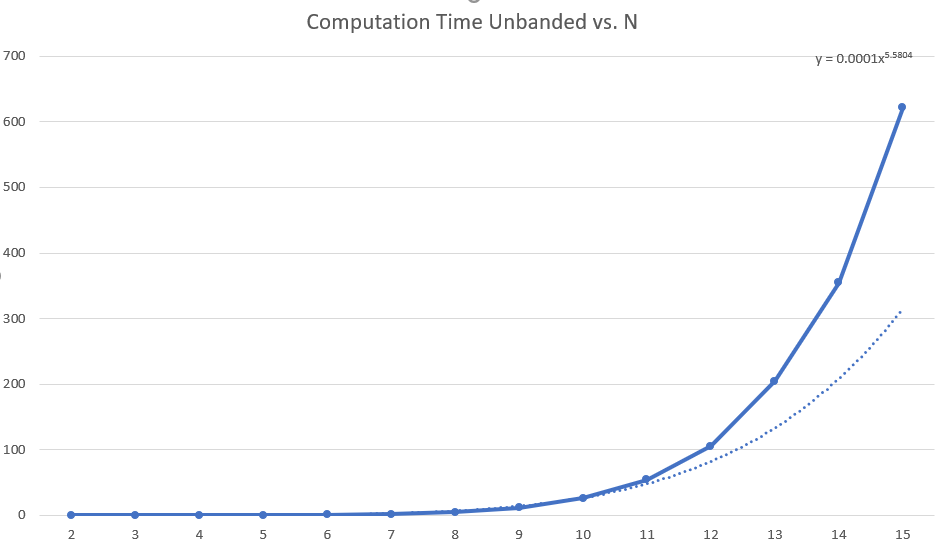
\includegraphics[width=\linewidth]{comp_time_unbanded}
				\caption{Mesh Resistance Calculation Time vs. N Unbanded}
				\label{comp_unbanded}
			\end{figure}
		
			Figure \ref{comp_unbanded} shows the computation time versus N. The formula found from the data is 
			$$
				t = 0.0001N^{5.58}
			$$
			The curve generally agrees with the theoretical time $O(n^6)$.
			
		\subsection{Sparse Matrix Computation Time}
			The theoretical computation time of a banded sparse matrix is $O(\bar{b}^2n)$. By relating with the mesh size, the time complexity becomes $O(N^4)$.
			\begin{figure}[!h]
				\centering
				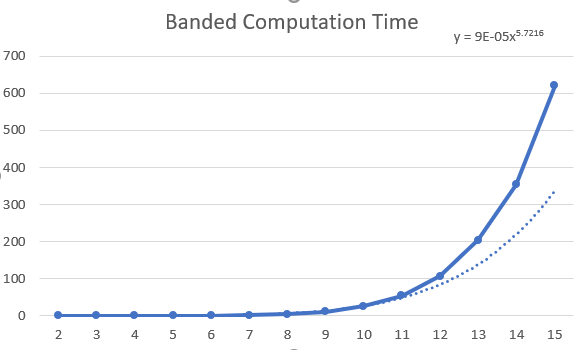
\includegraphics[width=\linewidth]{banded_time}
				\caption{Mesh Resistance Calculation Time vs. N banded}
				\label{comp_banded}
			\end{figure}
		
			Figure \ref{comp_banded} shows the computation time for banded solution. My result does not agree with the theoretical computation time. I consider that there exists a lot of overheads during computations which slows down the overall time. For example, when I am using the banded algorithm, I keeps checking if my element of interest is about to exceed my half-bandwidth, which can cause a very big process overhead. 
			
		\subsection{Resistance vs. Mesh Size}
			Use the resistance computed by the program, plot the resistance $R$ vs. $N$. Figure \ref{mesh_re} shows the resistance changes versus the change of the mesh size. The formula derived from this data set is found to be 
			$$
				R = 9880.3log(N)+8452.9
			$$
			\begin{figure}[!h]
				\centering
				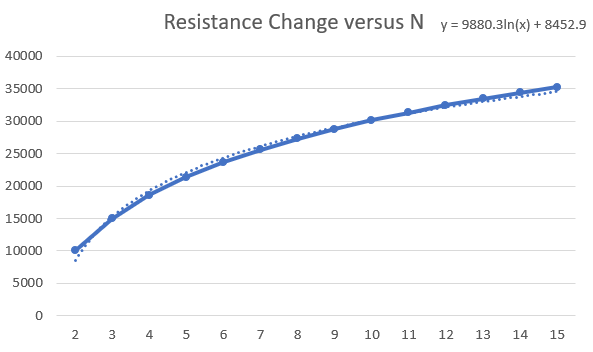
\includegraphics[width=\linewidth]{mesh_resistance}
				\caption{Mesh Resistance}
				\label{mesh_re}
			\end{figure}
	\section{Finite Difference for the Coaxial Cable}
		\subsection{Implementation of SOR}
			Method \mintinline{python}{successive_over_relaxation} in Listing \ref{lst:fd} shows the implementation of successive over relaxation for the coaxial cable.
			
			By using the symmetry of the problem. the implemented program constructs the quarter in the second quadrant of the cable. By doing this, the memory required to run the program is quartered.
			
		\subsection{Effects of Varying $\omega$}
			Fix the node distance $h = 0.02$, run the implemented program to get the voltage at $(0.06, 0.04)$. Because of symmetry, the program computes the value of the voltage at $(0.06, 0.16)$, which equals to the value at $(0.06, 0.04)$. Figure \ref{iteration_omega} shows how the number of iterations change with the change of $\omega$. From the graph, we can tell that the optimal $omega$ has a value of $1.3$ since the number of iterations reaches the lowest point of 26 iterations.
			\begin{figure}[!h]
				\centering
				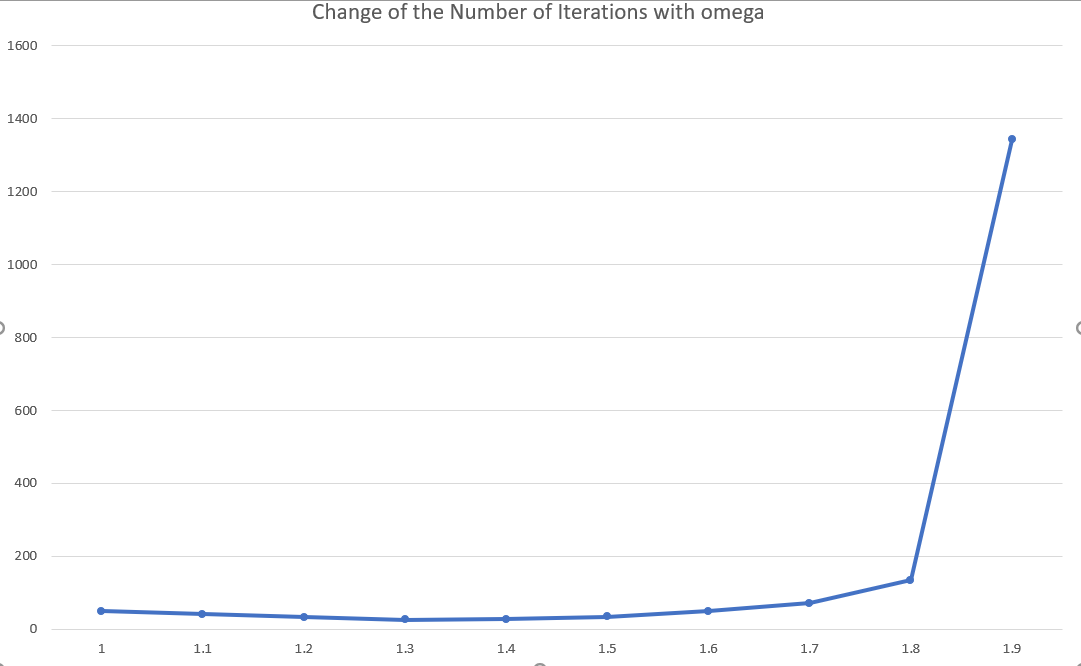
\includegraphics[width=\linewidth]{iteration_omega}
				\caption{Change of Number of Iterations with $\omega$}
				\label{iteration_omega}
			\end{figure}
		\subsection{Effects of Varying $h$}
			With the optimal point $\omega = 1.3$, vary the distance between the nodes. From $h = 0.02$, decrease the distance by a factor of 2, until $h = 0.00125$. The data recorded are shown in Table \ref{table:h_result}, and the plots are shown in Figure \ref{vol_1h_sor} and \ref{iter_1h_sor}.
			
			\begin{table}[!htb]
				\centering
				\caption{Potential at (0.06, 0.04) versus $h$ when using the SOR method.}
				\csvautobooktabular{../h_result.csv}
				\label{table:h_result}
			\end{table}
			\begin{figure}[!h]
				\centering
				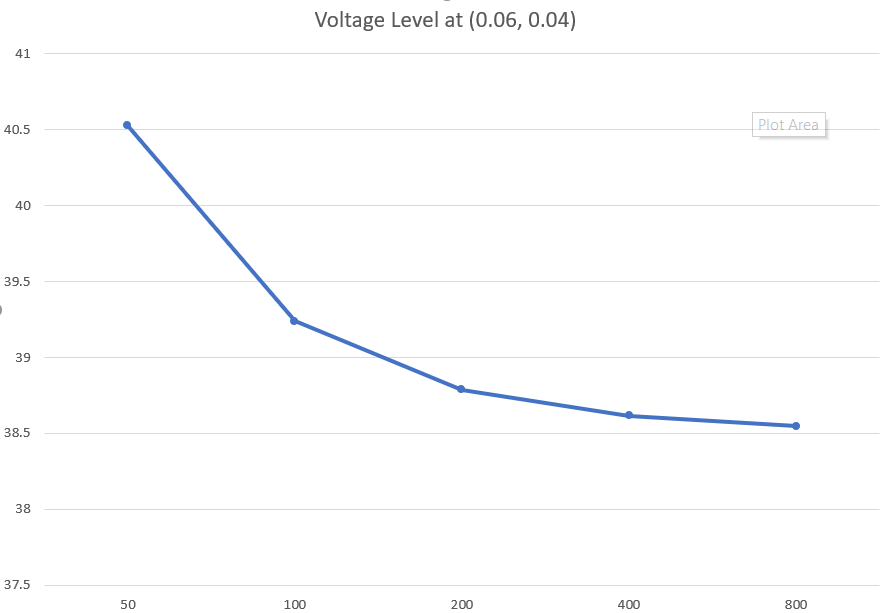
\includegraphics[width=\linewidth]{vol_1h_sor}
				\caption{Change of Voltage Levels versus 1/h}
				\label{vol_1h_sor}
			\end{figure}
			\begin{figure}[!h]
				\centering
				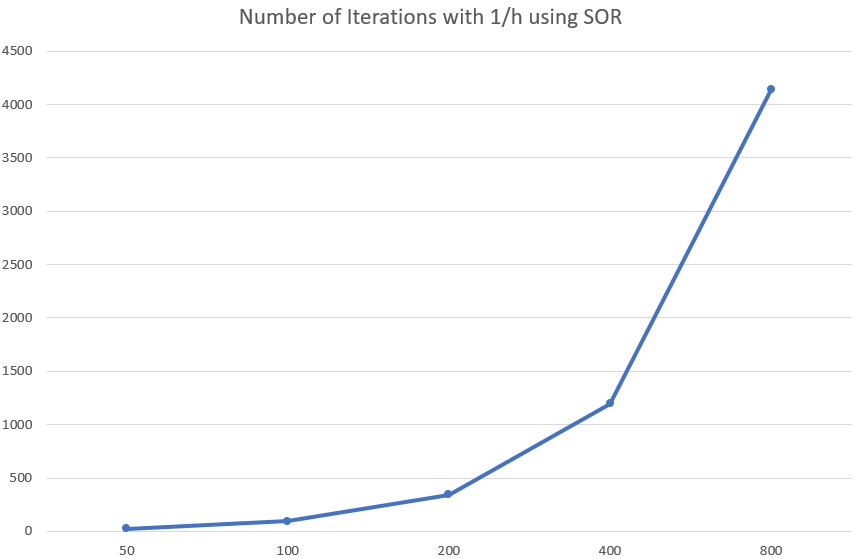
\includegraphics[width=\linewidth]{iter_1h_sor}
				\caption{Number of Iterations versus 1/h}
				\label{iter_1h_sor}
			\end{figure}
		
			From the two figures above, we can see that the precision of the calculation result is increasing, with the price of a very big increase in the calculation time. Therefore, a trade-off decision should be made to decide if the increase of time is well-worthy for the precision. As far as I am concerned, the precision using $h = 0.005$ is enough for the purpose of getting a general idea of the voltage level. After $h = 0.005$, the increase in precision is limited, while the computation time sky-rockets.
		\subsection{Varying $h$ using the Jacobi Method}
			In Listing \ref{lst:fd}, the method \mintinline{python}{jacobi} implements the Jacobi method. Export the computing results to a $.csv$ file, and the results are shown in Table \ref{table:h_jacobi_result}, and the plots of iterations and voltage levels are shown in Figures 
			\begin{table}[!htb]
				\centering
				\caption{Potential at (0.06, 0.04) versus $h$ when using Jacobi method.}
				\csvautobooktabular{../h_jacobi_result.csv}
				\label{table:h_jacobi_result}
			\end{table}
			\begin{figure}[!h]
				\centering
				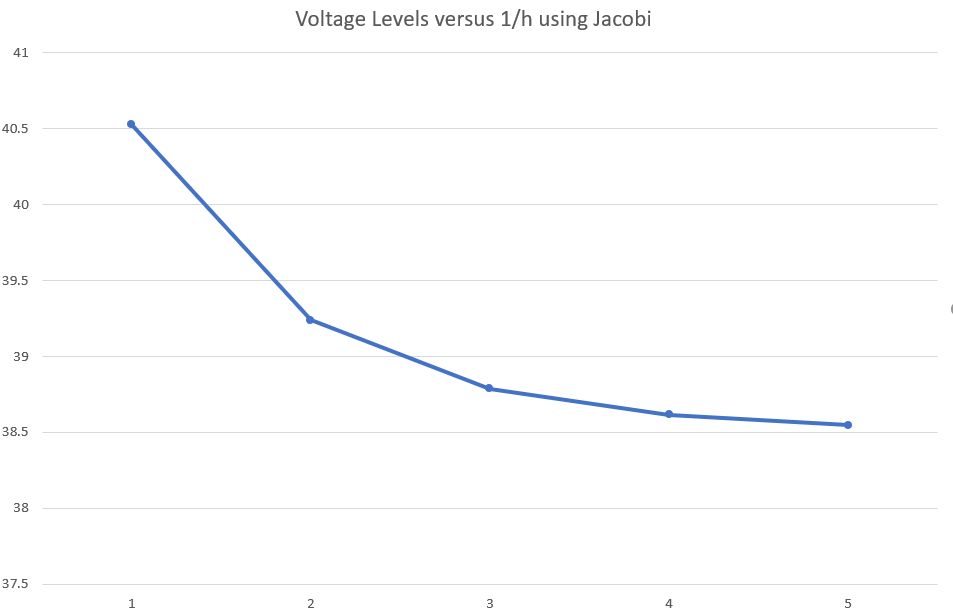
\includegraphics[width=\linewidth]{vol_1h_jacobi}
				\caption{Change of Voltage Levels versus 1/h using Jacobi Method}
				\label{vol_1h_jacobi}
			\end{figure}
			\begin{figure}[!h]
				\centering
				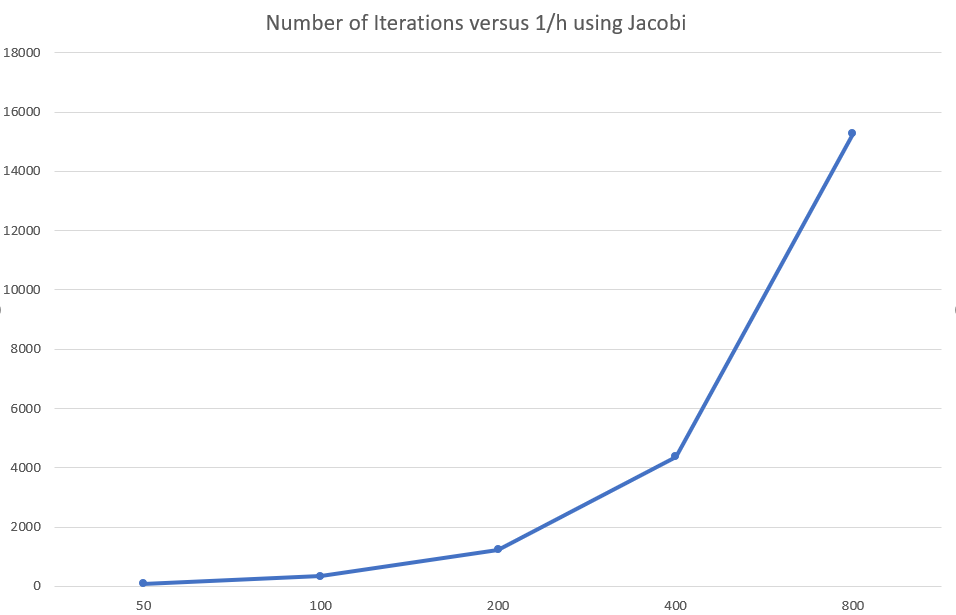
\includegraphics[width=\linewidth]{iter_1h_jacobi}
				\caption{Number of Iterations versus 1/h using Jacobi Method}
				\label{iter_1h_jacobi}
			\end{figure}
			
			From the two graphs, we can easily tell that the final calculated value is valid using Jacobi Method, but meanwhile it consumes much more computational time comparing with the successive over relaxation method. Similar to the SOR method, with the increase of precision (decrease of nodal distance), the computation time grows very rapidly. 
											
	\onecolumn
	\begin{appendices}
		
		\section{Code Listings} \label{appendix:code}
		
		\setminted{linenos,breaklines,fontsize=\footnotesize}
		
		\begin{center}
			\captionof{listing}{Custom matrix package (\texttt{matrix.py}).}
			\inputminted{python}{../matrix.py}
			\label{lst:matrices}
		\end{center}
		
		\begin{center}
			\captionof{listing}{Choleski decomposition (\texttt{choleski.py}).}
			\inputminted{python}{../choleski.py}
			\label{lst:choleski}
		\end{center}
		
		\begin{center}
			\captionof{listing}{Linear resistive networks (\texttt{linear\_networks.py}).}
			\inputminted{python}{../linearNetwork.py}
			\label{lst:linear_networks}
		\end{center}
		\begin{center}
			\captionof{listing}{Finite Difference (\texttt{finite\_difference.py}).}
			\inputminted{python}{../finite_difference.py}
			\label{lst:fd}
		\end{center}
		
	\end{appendices}
	

\end{document}